\documentclass[letterpaper,conference,fleqn]{IEEEtran}
%\documentclass[11pt,letterpaper,conference,fleqn]{IEEEtran}

\usepackage{times,epsfig,graphicx,cite,subfig,mathtools,amssymb}
\usepackage{url}

\DeclarePairedDelimiter\ceil{\lceil}{\rceil}
\DeclarePairedDelimiter\floor{\lfloor}{\rfloor}

% \pagestyle{empty}
%       \setlength{\parskip}{12pt}
%       \renewcommand{\baselinestretch}{1.1}

\begin{document}

% ------------------------------------------------------------
%\newcommand {\softNewpage}     {\newpage}
\newcommand {\softNewpage}      {}

%\newcommand* {\OmitProof} {}            % Expose this line to omit the
     % \ifdefined\OmitProof		% part after else
     % ...
     % \else
     % ...
     % \fi
% ------------------------------------------------------------
\newtheorem{lemma}{Lemma}
% \newtheorem{thm}{Theorem}
\newtheorem{thm}{{\break \noindent {\bf Theorem}}}

\newcommand{\loc}   	{ {\mathrm {Loc}} }
\newcommand{\ACONN}   { {\mathrm {A\mbox{-}CONN}} }
\newcommand{\SCONN}   { {\mathrm {S\mbox{-}CONN}} }

\newcommand{\fConn}   	{ {\mathrm {Conn}} }

\newcommand{\nReq}    { {n_{req}} }
\newcommand{\boldS}   { \mathbf{S}}
\newcommand{\DCH}     { {DCH} }

%% -- older paper --

\newcommand{\starEqual}   { {\;{\scriptstyle *} \! =} }
\newcommand{\plusEqual}   { {\;{\scriptstyle +} \! =} }
%\newcommand{\plusplus}    { {\scriptstyle \!+\!+} }

%\newcommand{\starEqual}   { {\; {\mathtt *=}} }
%\newcommand{\plusEqual}   { {\; \mathtt{+=}} }

% --------------------
\newcommand{\set}[1]    {{ \{ #1 \} }}
\newcommand{\iin}[1]    {\hspace*{#1in}}

\newcommand{\ol}[1]     {\overline{#1}}

\newcommand{\Prob}[1]   { {\bf \mathrm{Prob}} \left[ #1 \right] }
\newcommand{\aPr}	{ {\mathrm  {Pr}} }

\newcommand {\nwline} {\hfill\break}
% ------------------------------------------------------------
%	\pagestyle{myheadings}
%	\markboth{{\tt {E. Elmallah (draft)} \hfill}}
%	          {{\tt {E. Elmallah (draft)} \hfill}}
%
%	\begin{minipage}[t]{4in} \vspace*{-.5in}
%	{\small \tt submitted to ....} \vspace{.5in}
%	\end{minipage}
%
% ------------------------------------------------------------
\title {
       Tree Bound on Probabilistic Connectivity of Underwater Sensor Networks
}
\author {
        \IEEEauthorblockN{Md Asadul Islam}
	\IEEEauthorblockA{
                Department of Computing Science \\
                University of Alberta \\
                Edmonton, T6G 2E8, Canada\\
                E-Mail: mdasadul@ualberta.ca
        }
	\and
        \IEEEauthorblockN{Ehab S. Elmallah}
	\IEEEauthorblockA{
                Department of Computing Science \\
                University of Alberta \\
                Edmonton, T6G 2E8, Canada\\
                E-Mail: elmallah@ualberta.ca
        }
}
%	\date{March 21, 2014}
%	\thanks{This research is supported by NSERC Canada under grant
%		number OGP 36899.}
\maketitle
\thispagestyle{empty}
% --------------------
%
\begin{abstract}
This paper considers Underwater Sensor Networks (UWSNs) with unanchored
nodes that can move freely with water currents.
%
Thus, node locations at any instant can only be specified probabilistically.
%
When connectivity among some of the sensor nodes is required to perform
a given function, the problem of estimating the likelihood that the network
achieves such connectivity arises.
%
Our work here formulates a parameterized probabilistic connectivity
problem that serves this purpose when the network contains both sensor nodes
and relay nodes.
%
We show an exact dynamic programming algorithm for solving the problem
on networks with tree-like structure; 
the algorithm yields lower bounds on the solution of
the problem on any arbitrary network.
%
The obtained simulation results investigate the gap between our obtained
lower bounds and exact solutions on small networks, as well as
the usefulness of our method in analyzing the effect of adding relay nodes
to the network.
\end{abstract}
%
% ------------------------------
\ifdefined\OmitProof
%
\else
\nwline
\begin{IEEEkeywords}
Underwater sensor networks,
probabilistic connectivity,
probabilistic graphs.
\end{IEEEkeywords}
\fi
% ------------------------------
% ------------------------------------------------------------

%\section{Introduction}  {\bf To be completed}

\section{Introduction}

% --------------------
%\begin{itemize}
%\item  Books: \cite{xiao2010underwater, otnes2012underwater}
%
%\item  Surveys: \cite{akyildiz2005underwater, partan2007survey,
%       climent2014underwater, heidemann2012underwater}
%
%\item  Architecture: \cite{jaffe2006sensor}
%
%\item  Real world: \cite{le2013realWorld, roy2006wideArea}
%\item  Coverage: \cite{senel2013auto, pompili:2006deploymen}
%
%\item  Reliability: \cite{Co87}
%\item  Delays: \cite{pu2013comparing}
%
%\item  Very related: \cite{bower1989evidence, bower91simple,
%       caruso2008meandering, luo2009double, elmallah01supporting}
%\end{itemize}
% --------------------

Research on Underwater Sensor Networks (UWSNs) has intensified in recent
years.
Interest in such research has been fueled by many important underwater
sensing applications and services that can be supported by such networks
(see, e.g., \cite{akyildiz2005underwater,heidemann2012underwater}).
%
The domains of such applications are diverse and can be roughly classified as
scientific applications (e.g., collecting data on geological processes,
analyzing water characteristics, study of marine life),
industrial applications (e.g., monitoring underwater equipment and pipelines
used in oil industry),
humanitarian applications (e.g., search and survey missions, prediction of
natural disturbances) and/or
military and home land security applications (e.g., securing port facilities).

To serve the above diverse types of applications, various types
of UWSN deployments are used.
%
In \cite{heidemann2012underwater}, for example, UWSN deployments are
classified as being either static, semi-mobile, or mobile.
%
Static networks have nodes attached to underwater ground,
anchored buoys, or docks.
%
Semi-mobile networks may have collection of nodes attached to a
free floating buoy. Nodes in semi-mobile networks are subject to small scale
movements.
%
Mobile networks may be composed of drifters with no self mobility
capability, or nodes with mobility capability. Nodes in such networks
are subject to large scale movements.
%
UWSN deployments may occur over many short periods of times (e.g.,
several days at a time), so as to conduct several missions over
a large area of interest.
%

Due to the importance of such applications, and the challenges encountered
in their design, extensive work spanning all five layers of the Internet
protocol stack appear in the literature.
%
See, e.g., the chapters in \cite{xiao2010underwater, otnes2012underwater},
and the survey articles in \cite{partan2007survey, climent2014underwater}.
%
Examples of real-world UWSN work include
\cite{rice2000evolution,jaffe2006sensor,roy2006wideArea,rice2007seaweb,
pu2013comparing}.

% ------------------------------
In this paper, we consider semi-mobile and mobile networks.
%
Maintaining connectivity in such networks is a crucial aspect for
any task requiring node collaboration.
%
Our interest in on developing methodologies that allow a designer
to analyze the likelihood that a network (or part of it) is connected
at a given time interval.

For literature review, we note that several experimental and analytical
results in oceanography literature have shaped our current understanding
of mobility for underwater sensor networks.
%
Of the vast literature existing in the field, we recall the following
early landmark results.
%
In \cite{bower1989evidence}, the authors report on several observations
collected in the Gulf Stream using thirty-seven RAFOS drifters launched
off Cape Hatteras. Mobility of the free floating drifters are tracked
for 30 or 45 days.
%
In \cite{bower91simple}, the author describes a 2-dimensional kinematic
model of a meandering jet. 
%
The model captures the striking patterns of cross-stream and vertical
motion associated with meanders observed in \cite{bower1989evidence}.


Investigations and results obtained in the above directions have
been valuable for networking researchers approaching the challenge
of modelling the mobility of underwater sensor networks.
%
In \cite{caruso2008meandering}, the authors adopt a kinematic model
for capturing the effect of meandering sub-surface currents and v̰o̰r̰t̰ḭc̰ḛs̰
of free floating sensor nodes.
%
The model, called the meandering current mobility model, is useful
for large coastal environments that span several kilometers.
%
It captures the strong correlations in mobility of nearby sensor nodes.
%
Using simulation, the authors investigate several network connectivity,
coverage, and localization aspects.


In \cite{luo2009double}, the authors consider sensor nodes with movement
capability.
%
Each node incurs both uncontrollable and controllable mobility
(abbreviated as U-mobility and C-mobility).
%
Using a grid layout that divides a geographic area into cells, the authors
adopt a probabilistic U-mobility model.
%
The model takes into consideration two types of effects:
{\em local variety} effects (caused by reefs, turbulence), and
{main circulation}  effects (caused by wind, salinity).
%
Using such model, the authors present an energy efficient approach for
satisfying network coverage requirements.


In this paper, we adopt a simple {\em probabilistic locality} model
where the geographic area under consideration is partitioned into
disjoint regions (rectangles) using a grid layout.
%
In our model, the use of a high grid resolution (i.e., a layout with small
regions) can potentially give accurate results at the expense of decreased
solution efficiency.
%
We assume that one can utilize a physical model of underwater currents to
compute the probability that a sensor node is located at a given region
during some time interval of interest.
%
For example, one may utilize the kinematic model adopted in
\cite{caruso2008meandering} to compute such probabilities from a
sufficiently large number of node trajectories generated by the model.
%
Using such probability distribution, one obtains a {\em probabilistic} graph
model of the network.

Our work here formalizes two problems, denoted $\ACONN$ and $\SCONN$,
that call for determining the likelihood that a probabilistic graph
is entirely or partially connected.
%
Our main contribution is an efficient dynamic programming algorithm to
solve both problems on tree-like networks.
%
The algorithm can be used to derive lower bounds on the solution of
any arbitrary probabilistic network.
%
Our devised algorithm extends a result in \cite{elmallah01supporting}
to compute the probability that a given sequence of nodes 
in a probabilistic network forms a simple connected path.
%
To the best of our knowledge, both the problems formulation and devised
algorithm are novel aspects of the paper.  

In the next two sections we outline the system model and problem formulations.
Section 4 then gives a detailed description of the algorithm.


%\newpage

\section{Network Model}

In this section, we present a network model that deals with UWSNs with
arbitrary topologies where node location is described probabilistically.
%
In addition to using sensor nodes, the model allows networks to utilize
relaying nodes that do not perform sensing functions, but can enhance
the overall network connectivity.

% ------------------------------
\subsection{Node Locality Sets}

We denote by $V= V_{sense} \bigcup V_{relay}$ the set of nodes in
a given UWSN $G$ where $V_{sense}$ is a subset of sensor nodes that
can perform both sensing and data communication, and $V_{relay}$ is
a subset of relay only nodes that do not perform sensing.
%
We assume that $V_{sense}$ has a distinguished {\em sink} node,
denoted $s$, that performs network wide command and control functions.


After some time interval $T$ from network deployment time,
each node $x$ can be in some location determined by water currents
causing node movement.


To simplify analysis, approaches in the literature typically divide
the geographic area containing nodes into rectangles of a superimposed
grid layout.
%
Thus, at time $T$, each node $x$ can be in any one of a possible
set of grid rectangles denoted $\loc(x)= \{ x[1], x[2], \cdots \}$.
%
We call $\loc(x)$ the {\em locality} set of $x$ (for simplicity,
we omit the dependency on $T$ from the notation).
%
Depending on the mobility model induced by water currents, node $x$
can be in any possible grid rectangle $x[i]$ with a certain probability,
denoted $p_x[i]$. 
%
Computing such probability distribution is outside the scope of the paper.
We assume, however, that such distribution is computable given enough
information on the dynamical aspects of the water currents.

Henceforth, we use $x[i]$ to refer to node $x$ at the $i$th location index.
%
For brevity, we also refer to $x[i]$ as the location of $x$
(rather than the grid rectangle containing $x$) at an instant of interest.
%
To gain efficiency in solving large problem instances with large locality
sets, it may be convenient to truncate some locality sets to include only
locations of high occurrence probability, and ignore the remaining locations.
%
In such cases, we get $\sum_{x[i] \in \loc(x)} p_x(i) \leq 1$, if $\loc(x)$
is truncated.

% ------------------------------
\subsection{Node Reachability}

At any instant, node $x$ can reach node $y$ if the acoustic signal strength
from $x$ to $y$ (and vice versa) exceeds a certain threshold value.
%
In acoustic UWSN, the directions of water currents play an important role
in signal delay (see, e.g., \cite{pu2013comparing}).
%
For simplicity, we assume that given the exact locations of $x$ and $y$,
we can determine if $x$ and $y$ can reach each other, and if so, we
set the link indicator $E_G (x,y)= 1$.
%
Else, if no satisfactory communication can take place then
we set $E_G (x,y)= 0$.


Our general objective in this paper is to develop effective methodologies
for computing lower bounds on the likelihood that the network is totally,
or partially, connected.
%
To this end, we adopt the following rule: we set $E_G(x[i],y[j])= 1$
if and only if the two nodes $x$ and $y$ can reach each other if
they are located anywhere in their respective rectangles $x[i]$ and $y[j]$.


The above rule implies that connectivity between $x$ and $y$ is ignored if 
they can reach each other at some (but not all) pairs of points in their
respective rectangles.
%
As can be seen, ignoring connectivity in such cases results
in computing lower bounds on the network connectivity, as required.
%
Our devised algorithm presented below is {\bf exact} with respect to
the given relation $E_G$ that defines the input network $G$.

% ------------------------------

\section{Problem Formulation}

We now introduce two fundamental probabilistic connectivity problems
on any given UWSN $G= (V= V_{sense} \bigcup V_{relay}, E_G, \loc, p)$.
%
The first problem is the {\em all} sensor node connectivity problem:

\nwline
{\bf Definition (the $\ACONN$ problem).}
    Given an UWSN $G$, compute the probability $Conn(G)$ that the network
    is in a state where the sink node $s$ can reach all sensor nodes.     
\IEEEQED

\nwline
The second problem is the {\em subset} sensor node connectivity problem:

\nwline
{\bf Definition (the $\SCONN$ problem).}
    Given an UWSN $G$, and an integer $\nReq$, $\nReq \leq |V_{sense}|$,
    compute the probability $Conn(G,\nReq)$ that the network is in a state
    where the sink node $s$ can reach a subset of sensor nodes having at
    least $\nReq$ sensor nodes.
\IEEEQED

\nwline
Thus, the $\ACONN$ problem is an important special case of the $\SCONN$
problem where $\nReq= |V_{sense}|$.
%
We next remark that the above problems share some basic aspects
with the class of network reliability problems discussed in \cite{Co87}.
%
In particular, all such problems are defined over some type of probabilistic
graphs where each node (and/or link) can be in any one of two, or more,
states.
%
In case of network reliability problems, a node or link can either be
{\em operating} or {\em failed}, whereas in our present context, a node
can be in any one of a possible set of locations.
%

Events of interest on such probabilistic graphs occur when the given network
is in some particular {\em network states}.
%
In our present context, a network state $S$ of $G$ arises when each node
$x \in V$ is located at some specific location in its respective locality
set $\loc(x)$.
%
Thus, if $V = \{v_1, v_2, \cdots, v_n \}$ then a state $S$ of $V$ can be
specified by $\{ v_1[i_1], v_2[i_2], \cdots, v_n[i_n] \}$ where
each $v_\alpha [i_\alpha] \in \loc(v_\alpha)$.
%
Two states $S_1$ and $S_2$ are different if they differ in the location 
of at least one node.
%
Assuming node locations are independent of each other, we have
$\aPr(S)= \prod_{v_\alpha \in V} p_{v_\alpha} [i_\alpha]$.

In the $\ACONN$ problem, a sate is {\em operating} if the sink $s$
can reach all sensor nodes in $V_{sense}$.
%
Likewise, in the $\SCONN$ problem, a state $S$ is {\em operating} if
the sink node $s$ can reach a subset having at least $\nReq$ sensor nodes.
%
Let $\boldS$ be the set of all operating states $S$ of a given
$\ACONN$ or $\SCONN$ problem then the required solution is given by
$\sum_{S \in \boldS} \aPr(S)$.

    % ------------------------------
\vspace*{-0.15in}
    \begin{figure}[htbp]
    \begin{center}
    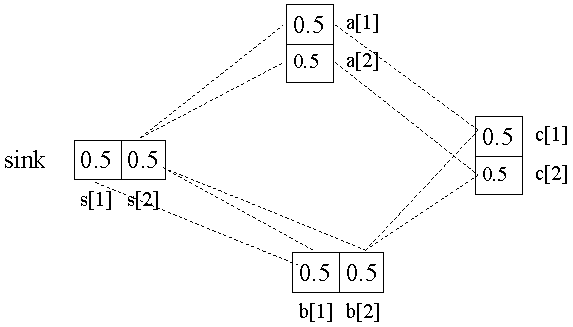
\includegraphics[width=2.75in]{4-node.pdf}
    \caption{An example network with locality sets}
    \label{fig:4node}
\vspace*{-0.25in}
    \end{center}
    \end{figure}
    % ------------------------------

\nwline
{\bf Example.}
     Fig.~\ref{fig:4node} illustrates a probabilistic graph on 4 nodes
     where $V= \{s, a,b,c\}$, and the locality set of each node has 2
     locations.
     %
     The network has $2^4$ states.
     %
     For the $\ACONN$ problem, 
     state $S_1= \{ s[2], a[2], b[2], c[2] \}$ is operating, and
     state $S_2= \{ s[1], a[1], b[1], c[2] \}$ is failed.
\IEEEQED
% ------------------------------
% ------------------------------------------------------------




%\section{Main Algorithm} {\bf To be completed}

\section{Exact Tree Algorithm}

In this section, we first identify a class of probabilistic networks
that have tree-like topologies.
%
Next, we present an efficient algorithm that computes the exact
$Rel(G,\nReq)$ on such class of networks.
%
Our algorithm is conceptually simple, and the design is optimized to
solve the $\ACONN$ problem so as to alleviate the need for implementing
a restricted version of the algorithm.
% ------------------------------

\subsection{Probabilistic Networks with Tree T̠o̠p̠o̠l̠o̠g̠i̠e̠s̠}

To start, we say that a probabilistic network $G=(V,E_G,\loc,p)$ has
the topology of a conventional tree $T=(V,E_T)$ if whenever $E_G(x[i],y[j])= 1$
then $(x,y) \in E_T$.
%
Note that the definition allows two nodes $x$ and $y$ to be adjacent in
$T$, and yet they can take positions, say $x[i]$ and $y[j]$, such that
$E_G (x[i],y[j])= 0$.
%
Thus, each state $S$ of $G$ gives the tree $T$ with possibly some missing
links.

\nwline
In any such tree network $G$, one may safely delete a relay node
$x \in V_{relay}$ that appears as a leaf node without changing the problem
solution. 
%
This observation holds since relay nodes are relevant only if they
connect some sensor node to the sink $s$.
%
We henceforth assume, without loss of generality, that the input tree
network $G$ has no relay leaf.
% ------------------------------

\subsection{Overview of the Algorithm}

The algorithm (Function $\fConn$ in Fig.~\ref{alg:Conn}) employs a
dynamic programming approach.
%
It takes as input an instance $(G,\nReq)$ of the $\SCONN$ problem,
and a tree $T=(V,E_T)$ on the set $V$ of nodes with no relay leaves.
%
The function computes the exact solution $Conn(G,\nReq)$ of the given
instance.

We consider $T$ as a tree rooted at the sink $s$. Each node $y$ in $T$
has a parent node $x$ on the unique path from $y$ to the root $s$.
%
Each such node $y$ is a root of a subtree, denoted $T_y$, obtained by
removing the link $(y, parent(y))$ from $T$.


The key variables and data structures in the function are as follows.

\begin{itemize}
\item	$type(x)$:
	For any node $x$, $type(x)= 0$ if $x$ is a relay node,
	and $type(x)= 1$ if $x$ is a sensor node.

\item	$n_x$ ($=n_{x,sense} + n_{x,relay}$):
	$n_x$ is the total number of sensor nodes $n_{x,sense}$ and
	relay nodes $n_{x,relay}$ in subtree $T_x$ (including node $x$)

\item	$n_{x,min}$:
	The minimum number of sensor nodes in $T_x$ that should be connected
	to the sink in any operating state of the network.
	%
	So, $n_{x,min}= \max(0, \nReq - (n_{sense} - n_{x,sense}))$.
	Here, $n_{sense} - n_{x,sense}$ is the number of available sensor nodes
	not in $T_x$, and thus $\nReq - (n_{sense} - n_{x,sense})$,
	if non-negative, is the minimum number of sensor nodes of $T_x$
	required in any operating state of the network.
	%
	% That is, $n_{x,min}$ is the minimum contribution of tree $T_x$ to
	% any operating state of the network.

\item	$count_{x,min}$:
	The minimum number of sensor nodes in the part of $T_x$ processed
	thus far that should be connected to the sink in any operating state
	of the network.

\item	$\DCH(x)$:
	Each iteration of the main loop in Step 2 identifies
	a non-sink leaf node $y$ whose parent is denoted $x$. 
	The function then processes, and then deletes node $y$.
	Thus, in any iteration, each node $x$ may have some of its children
	processed and deleted.
	We denote such set of $x$'s deleted children by $\DCH(x)$.

\item	Tables $R_x$ (and $R'_x$):
	Each node $x \in V$ is associated with a table $R_x$.
	The table stores {\em key-value} mappings.
	%
	Each key is a pair $(i,count)$ where $i$ is a possible location
	index of $x$, and $count$ is a number of sensor nodes that are
	descendants of $x$ (including $x$ itself) in the graph processed
	thus far.
	%
	Roughly speaking, at any iteration of the main loop,
	$R_x(i,count)$ is the probability of obtaining a state over
	the subset of nodes in $T_x$ processed in previous iterations
	where $x[i]$ reaches exactly $count$ sensor nodes in such subset of
	$T_x$. 

\end{itemize}

% ------------------------------
    % --------------- Function E2P ---------------
    \begin{figure}[htbp]
    % \begin{figure}[!ht]
    \small
\begin{center}
\fbox{
    \begin{minipage}[t]{3.3in}
    \renewcommand{\baselinestretch}{1}
    %
    {\bf Function $\fConn (G, T, \nReq)$}
\nwline
	{\bf Input:}
	\begin{minipage}[t]{2.75in}
	An instance of the $\SCONN$ problem where $G$ has a tree
	topology $T$ with no relay leaves
	\end{minipage}
%
\nwline
	{\bf Output:}
	\begin{minipage}[t]{2.75in}
	$Conn(G, \nReq)$
	\end{minipage}
	\\
%
%\nwline
%	{\bf Notation:}
%	\begin{minipage}[t]{2.75in}
%	\end{minipage}
% --------------------
   \nwline
% initialization
   1.  \begin{minipage}[t]{3.00in}
       {\bf foreach} (node $x$ and a valid location index $i$) \\
       \{ \\
         \iin{0.20} set $R_x(i, type(x) )= 1$ \\
         \iin{0.20} $n_{x,min}= \min (0, \nReq - (n_{sense} - n_{x,sense}) )$ \\
       \}
       \end{minipage}
       \\
   \nwline       
% main loop
   2.  \begin{minipage}[t]{3.00in}
       {\bf while} ($T$ has at least 2 nodes) \\
       \{
       \end{minipage}
       \\
   3.  \iin{0.20} \begin{minipage}[t]{2.80in}
   		  Let $y$ be a non-sink leaf of $T$, and $x= parent(y)$
		  \end{minipage}
		  \\
   4.  \iin{0.20} \begin{minipage}[t]{2.80in}
   		  {\bf foreach} (key $(i,count) \in R_y$)
		       $R_y (i,count) \starEqual p_y[i]$
		  \end{minipage}
		  \\
   5.  \iin{0.20} \begin{minipage}[t]{2.80in}
   		  set $R'_x= \phi$
		  \end{minipage}
		  \\
   6.  \iin{0.20} \begin{minipage}[t]{2.80in}
   		  {\bf foreach} (pair of keys
		       		$\begin{array}[t]{l}
				 (i_x, count_x) \in R_x \mbox { and }\\
		   		 (i_y, count_y) \in R_y)
				 \end{array}
				$ \\ 
		  \{
		  \end{minipage}
		  \\
   7.  \iin{0.40} \begin{minipage}[t]{2.60in}
   		  $count= \min (count_x + count_y, \nReq)$
		  \end{minipage}
		  \\
   8.  \iin{0.40} \begin{minipage}[t]{2.60in}
   		  $count_{x,min}= \begin{array}[t]{l}
		  		  type(x) + n_{y,min} + \\
		       	   	  \sum_{z \in \DCH(x)} n_{z,min}
				  \end{array}$
		  \end{minipage}
		  \\
   9.  \iin{0.40} \begin{minipage}[t]{2.60in}
   		  {\bf if} ($count < count_{x,min}$) {\bf continue} 
		  \end{minipage}
		  \\
   10.  \iin{0.35} \begin{minipage}[t]{2.60in}
   		  $R'_x (i_x,count) \plusEqual$ 
		  	$\begin{array}[t]{l}
			 R_y(i_y,count_y) \times \\
			 R_x(i_x,count_x) \times \\
			 E_G(x[i_x], y[i_y])
		  	 \end{array}$
		  \end{minipage}
		  \\
       \iin{0.40} \} \\
   11. \iin{0.20} \begin{minipage}[t]{2.60in}
       		  set $R_x= R'_x$; remove $y$ from $T$
		   \end{minipage}
		   \\
       \iin{0.15} \} \\
   12. \begin{minipage}[t]{3.00in}
       return $\sum_{x[i] \in \loc(x)} R_s(i,\nReq) * p_s[i]$
       \end{minipage}
       \\
    \end{minipage}	
}
\end{center}
    \normalsize
    %
    \caption{Pseudo-code for function $\fConn$}
    \label{alg:Conn}
\vspace*{-0.1in}
    \end{figure}
    % ------------------------------

\subsection{Main Steps}

Step 1 initializes table $R_x$ for each node $x$ as follows.
%
For each possible location index $i$ of $x$, set $R_x(i, count=1)= 1$
if $x$ is a sensor node.
Else ($x$ is a relay node), set $R_x(i, count=0)= 1$.
%
Step 1 also initializes $n_{x,min}$.


Steps 2-11 form the main loop of the function.
The loop iteratively finds a leaf node $y$ that is not the sink $s$, 
processes node $y$, and then removes $y$ from the tree $T$.
%
Processing a node $y$ with parent $x$ is done as follows.

Step 4 updates each entry $R_y (i,count)$ by multiplying the entry
with $p_y[i]$.
%
As can be seen, this update operation is done in the iteration that ends by
removing $y$.
%
Step 5 initializes the temporary table $R'_x$ to empty.


Steps 6-10: the loop in step 6 performs a {\em cross product} of tables
$R_x$ and $R_y$, storing the result in table $R'_x$.
%
In the cross product, each pair of possible keys $(i_x, count_x)$
and $(i_y, count_y)$ are processed.
%
More specifically, suppose that $x[i_x]$ can reach $count_x$ sensor nodes
in the part of $T_x$ processed thus far with probability $R_x(i_x,count_x)$.
%
Also, suppose that $y[i_y]$ can reach $count_y$ sensor nodes
in $T_y$ with probability $R_y(i_y,count_y)$.
%
Thus, if $x[i_x]$ reaches $y[i_y]$ (i.e., $E_G(x[i_x],y[i_y])$= 1)
then $x[i_x]$ can reach a total of $count= count_x + count_y$ nodes.


If $count > \nReq$ then Step 7 truncates $count$ to $\nReq$.
%
On the other hand, if $count < count_{x,min}$ (i.e., $count$ is below the
minimum number of nodes required to construct an operating state) then
Step 9 skips Step 10 and starts a new iteration.
%
Step 10 updates the probabilities accumulated in $R'_x(i_x,count)$. 


After exiting the main loop, the current tree $T$ contains only the
sink node $s$. Step 12 computes the solution $Conn(G,\nReq)$ from
the table $R_s$ associated with the sink $s$.
% ------------------------------

\subsection{Correctness}

To prove correctness, we first introduce the following notation and
definitions.
%
For a given node $x$, and iteration $r \in [1,n-1]$ of the main loop
in Step 2, we have the following:
%
\begin{itemize}
\item	$\DCH (x,r)$:
	The set of $x$'s deleted children at the start of iteration $r$.

\item	$V_{x,deleted,r}$ ($= \bigcup_{y \in \DCH(x,r)} V_y$):
	The set of $x$'s deleted descendants at the start of iteration $r$.
\end{itemize}
%
For brevity, we omit $r$ when the iteration number is not important, or
understood by the context.


In the following definitions, $x$ is any node in $T$,
$i$ is a possible location index of $x$, and  $V_{x,delete}$ is
the set of deleted descendants associated with $x$ at the start of some
iteration.

\begin{enumerate}
\item[{\bf [D1]}]
    Let $S$ be a state over nodes in $\{ x \} \bigcup V_{x,delete}$.
    The {\em type} of $S$ is a pair $(i,count)$ where
    %
    \begin{itemize}
    \item   $x$ is at location $x[i]$
    \item   If $count = \nReq$ then the number of sensor nodes connected to
    	    $x[i]$ in $S$ is $\geq \nReq$
    \item   Else ($count < \nReq$), then the number of sensor nodes
    	    connected to $x[i]$ is $< \nReq$
    \end{itemize} 	   
\end{enumerate}

\begin{enumerate}
\item[{\bf [D2]}]
    We say that table $R_x$ is {\em complete} with respect to a given
    set $V_{x,delete}$ if the following conditions hold:
    %
    \begin{enumerate}
    \item  For each key $(i,count)$ in $R_x$, $R_x(i,count)$ is
    	   the probability of obtaining states over
	   $\{ x[i] \} \bigcup V_{x,delete}$ of type $(i,count)$.
	   (Before multiplying by $p_x[i]$, the probability is conditioned
	   on $x$ being at location $x[i]$).
    \item  Each key $(i,count)$ not in $R_x$ does not contribute to
    	   computing the solution $Conn(G,\nReq)$.
    \end{enumerate}
\end{enumerate}

\nwline
We now show the following theorem.

\begin{thm} \label{thm:correctness}
    At the start of each iteration of the main loop in Step 2,
    if $x$ is a node in the current tree $T$ then table $R_x$ is complete
    with respect to the associated set $V_{x,delete}$ of deleted nodes.
\end{thm}

\nwline
{\bf Proof.}
\nwline
{\bf Loop initialization:}
At the start of the 1st iteration, $T$ contains all nodes $V$, and
each node $x$ has $V_{x,delete}= \emptyset$.
%
Node $x$ in location $x[i_x]$ is associated with one state of type
$(i_x,count_x= 0)$ if $x$ is a relay node, or type
$(i_x,count_x= 1)$ if $x$ is a sensor node.
%
For each such state type, Step 1 correctly sets $R_x(i,count)$.

\nwline
{\bf Loop maintenance:}
Assume the theorem holds for all possible iterations $r$, where $r \leq n-2$.
We show that it holds in iteration $r+1$.
%
Let $y$ be the leaf node deleted in iteration $r$, and $x= parent(y)$.
$R_x$ is the only table that may have changed between iterations
$r$ and $r+1$.
%
Thus, it suffices to show that $R_x$ is complete with respect to
$\{ x \} \bigcup V_{x,delete,r+1}$ at the start of iteration $r+1$.
%
To this end, we note the following in iteration $r$:
%
\begin{itemize}
\item  Step 4: this step adjusts the probability of each state type
       $(i,count)$ in $R_y$ by taking into account $p_y[i]$.
\item  Step 6: this loop exhaustively generates all state types over the
       set $V_y \bigcup V_{x,delete,r}$ where $V_y$ is a̠l̠l̠ nodes of
       the subtree rooted at node $y$.
\item  Step 9: this step discards all state types that can not be extended
       (by adding sensor nodes from the unprocessed part of the tree)
       to satisfy the $\nReq$ requirement.
\item  Step 10: this step updates the probability of $R'_x(i_x,count)$ by
       adding the right hand side when states of type $(i_x, count)$
       can be extended to operating states.
\end{itemize}
\IEEEQED

Following an argument similar to the loop maintenance argument, one can
show that at Step 12, table $R_s$ associated with the sink node is
complete with respect to all nodes $V$ in the network.
%
Thus, the function returns the required solution $Conn(G, \nReq)$.

% ------------------------------

\subsection{Running Time}

Let $n$ be the number of nodes in $G$, and $\ell_{max}$ be the maximum
number of locations in the locality set of any node.

% ----------
\begin{thm}
    Function $\fConn$ solves the $\SCONN$ problem in
    $O(n \cdot n_{req}^2  \cdot \ell_{max}^2)$ time
\end{thm}

\nwline
{\bf Proof.}
We note the following.
\begin{itemize}
\item   Step 1: storing the tree $T$, and computing $n_x$ and $n_{x,min}$
	for each node $x$, require $O(n)$ time.

\item	Step 2: the main loop performs $n-1$ iterations.
	Each of Steps 3, 5, and 11 can be done in constant time.

\item	Step 4: this loop requires $O(\nReq \cdot \ell_{max})$ time.

\item	Step 6: this loop requires $O(n_{req}^2 \cdot \ell_{max}^2)$ iterations.
	Steps 7, 8, 9, and 10 can be done in constant time.
\end{itemize}
Thus, the overall running time is determined by the main loop that
requires $O(n \cdot n_{req}^2  \cdot \ell_{max}^2)$ time.
\IEEEQED
% ----------
%
\nwline
\begin{thm}
    Function $\fConn$ solves the $\ACONN$ problem in
    $O(n \cdot \ell_{max}^2)$ time.

    % Overall: $O(n \cdot \ell_{max} + n \cdot \ell_{max}^2)$
\end{thm}

\nwline
{\bf Proof.}
It suffices to show that the main loop requires the above time.
%
In the $\ACONN$ problem, $\nReq= |V_{sense}|$, and all sensor nodes
in any subtree $T_y$ should be connected to the root $y$ in any
operating state.
%
So, in any iteration of the main loop, each table $R_y$ contains keys
$(i,count)$ for only one value of $count$ (the maximum value obtainable
from descendants of $y$ processed and removed thus far).
%
That is, the maximum length of any table is $\ell_{max}$ independent
of $\nReq$.
%
This gives the running time shown in the theorem. 
\IEEEQED



%\section{Simulation Results} {\bf To be completed}

\section{Simulation Results}

In this section, we present simulation results that explore
the following performance aspects of our devised algorithm:
%
\begin{itemize}
\item  the execution time of the algorithm,
\item  the optimality gap for solving the $\ACONN$ and $\SCONN$ problems, and
\item  the effect of using relay nodes.
\end{itemize}

To explore the optimality gap of the devised algorithm, we have implemented
an exhaustive algorithm for computing exact solutions.
%
The algorithm works by generating all possible network states
of a given probabilistic network.
%
The exhaustive algorithm has a complexity that grows exponentially with
the number of nodes in the network. However, it can process a graph
with 10, or fewer, nodes in a reasonable time.
%
Both of the exhaustive algorithm, and our devised tree algorithm
are implemented in C++ with the use of STL (Standard Template Library)
container classes.


\nwline
{\bf Maximum Spanning Trees.}
To use our devised algorithm for obtaining lower bounds on $Conn(G,\nReq)$
of a given network, we need to select a spanning tree.
%
Ideally, one would prefer to use a spanning tree that gives the best
possible lower bound.
%
Currently, however, this latter problem appears to be an open problem.
%
In the absence of a known algorithm to compute such an optimum tree,
we resort to using a heuristic algorithm.
%
The algorithm works as follows.
%
We associate with each link $(x,y) \in E_G$ a probability, denoted $p(x,y)$,
of having the link $(x,y)$ present, given the locality sets $\loc(x)$ and
$\loc(y)$.
%
We then seek to compute a spanning tree with the highest possible
product of link probabilities.
%
This latter problem can be solved efficiently by using a standard minimum
spanning tree algorithm.
%
The results discussed utilizes such maximum spanning trees.


\nwline
{\bf Test Networks.}
%
For simplicity of constructing test networks and analyzing the obtained
results, we assume that all nodes have the same transmission range
$R_{tr}$, and we set the $E_G$ relation according to the Euclidean
distance between the involved nodes.

We have experimented with networks of different sizes in the range
[10,20] nodes where each node has a locality set in the range $[2,8]$
rectangles.
%
Here, we present selected results using the two networks in
Fig.~\ref{sim:g10}, denoted $G_{10}$, and
Fig.~\ref{sim:g10r}, denoted $G_{10,3}$.
The selected results are representative of the important findings
observed when using other networks.
%
The network $G_{10}$ has 10 sensor nodes, where $v[1]$ is the sink node.
%
As indicated in Fig.~\ref{sim:g10}, node locality sets vary in the range
$[3,6]$ locations where each location is a grid square of unit side length.
%
The figure illustrates a subset of links in $E_G$ that occur when 
$R_{tr}= 6.5$ units.
%
To avoid cluttering the diagram, we omit the $(x,y)$-coordinates of the
locality sets.
%
The network $G_{10,3}$ adds 3 relay nodes to $G_{10}$.
%
The exhaustive algorithm for computing exact connectivity deals only
with the links shown in $G_{10}$ and $G_{10,3}$ (some links may not
arise if $R_{tr} < 6.5$).
%
Solid lines in the figures indicate the links used in a maximum spanning tree.

     % ------------------------------
     %\begin{figure}[!ht]
     \begin{figure}[htbp]
     \begin{center}
     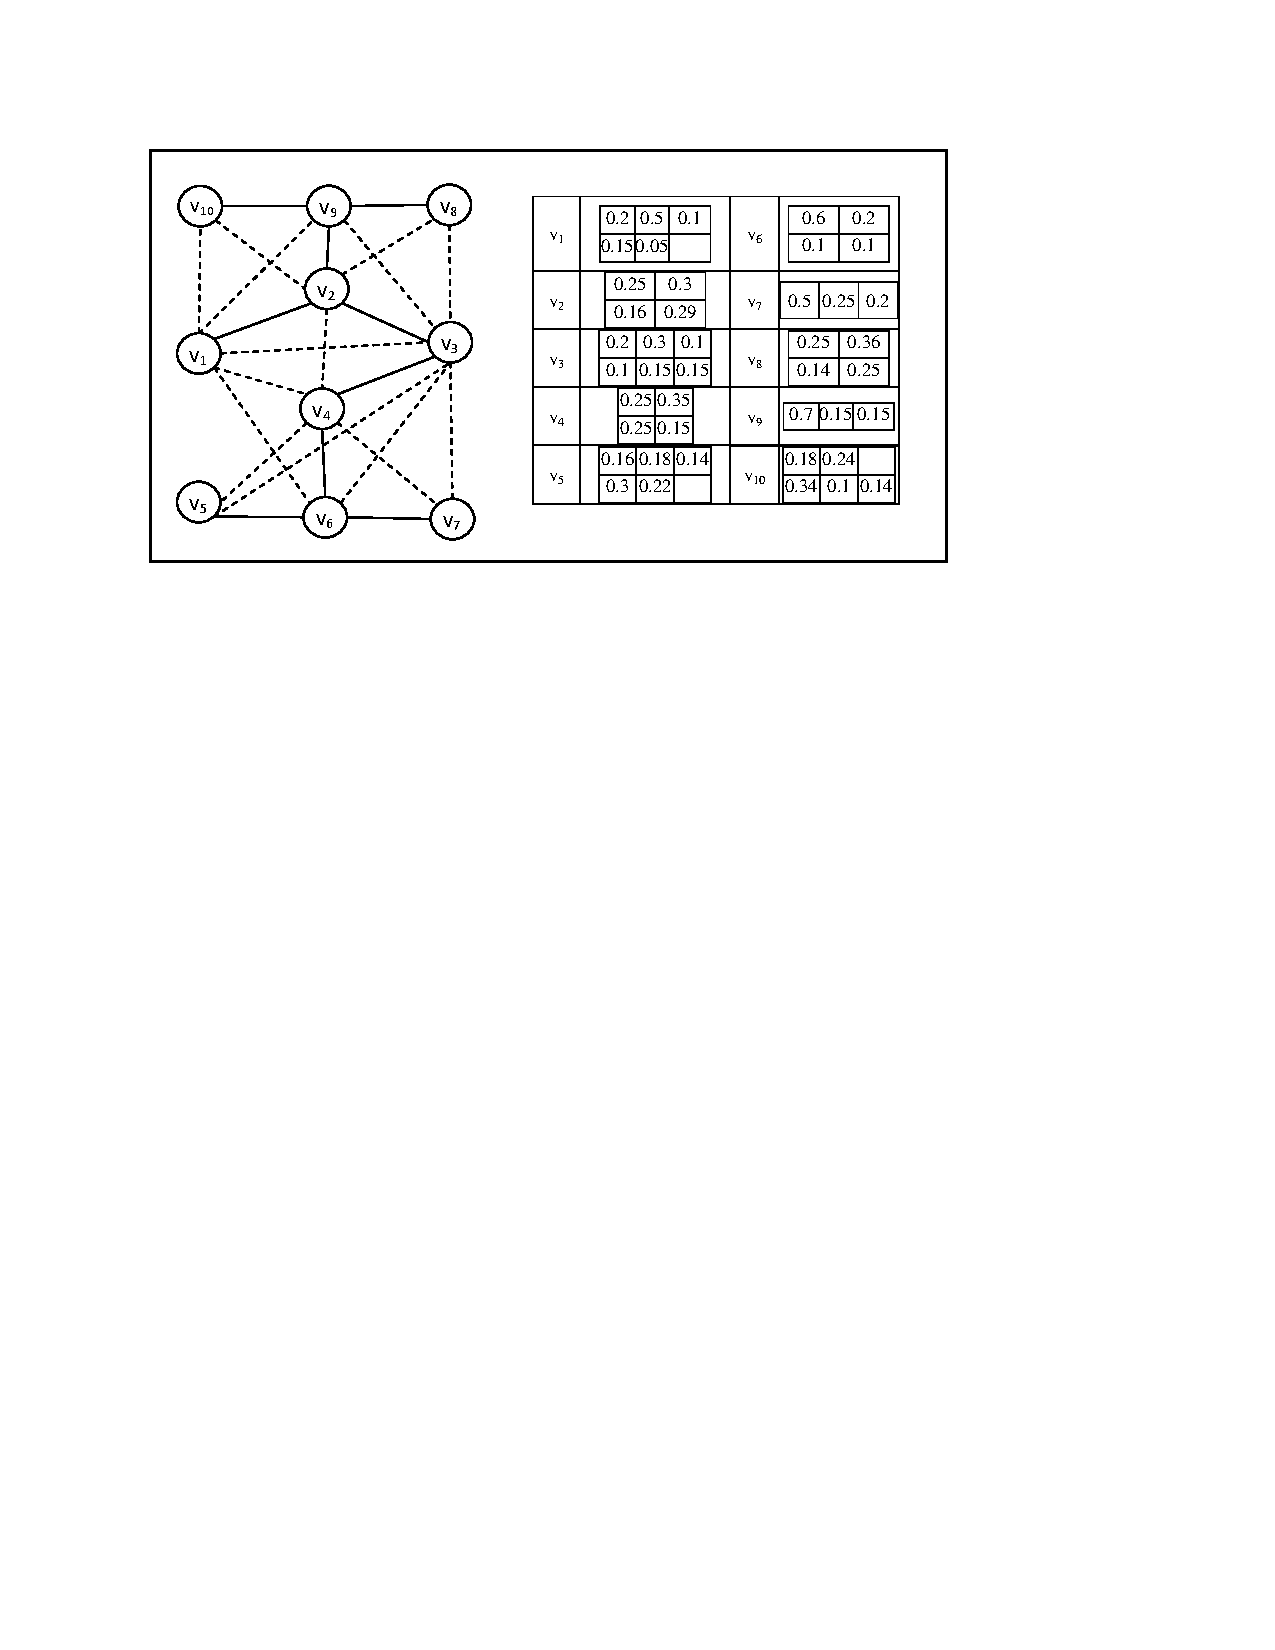
\includegraphics[width=3.3in]{g10.pdf}
     %
     % \caption{A probabilistic network on 10 nodes}
     \caption{The $G_{10}$ network}
     \label{sim:g10}
%\vspace*{-0.2in}
     \end{center}
     \end{figure}
     % ------------------------------
\vspace*{-0.2in}
     % ------------------------------
     %\begin{figure}[!ht]
     \begin{figure}[htbp]
     \begin{center}
     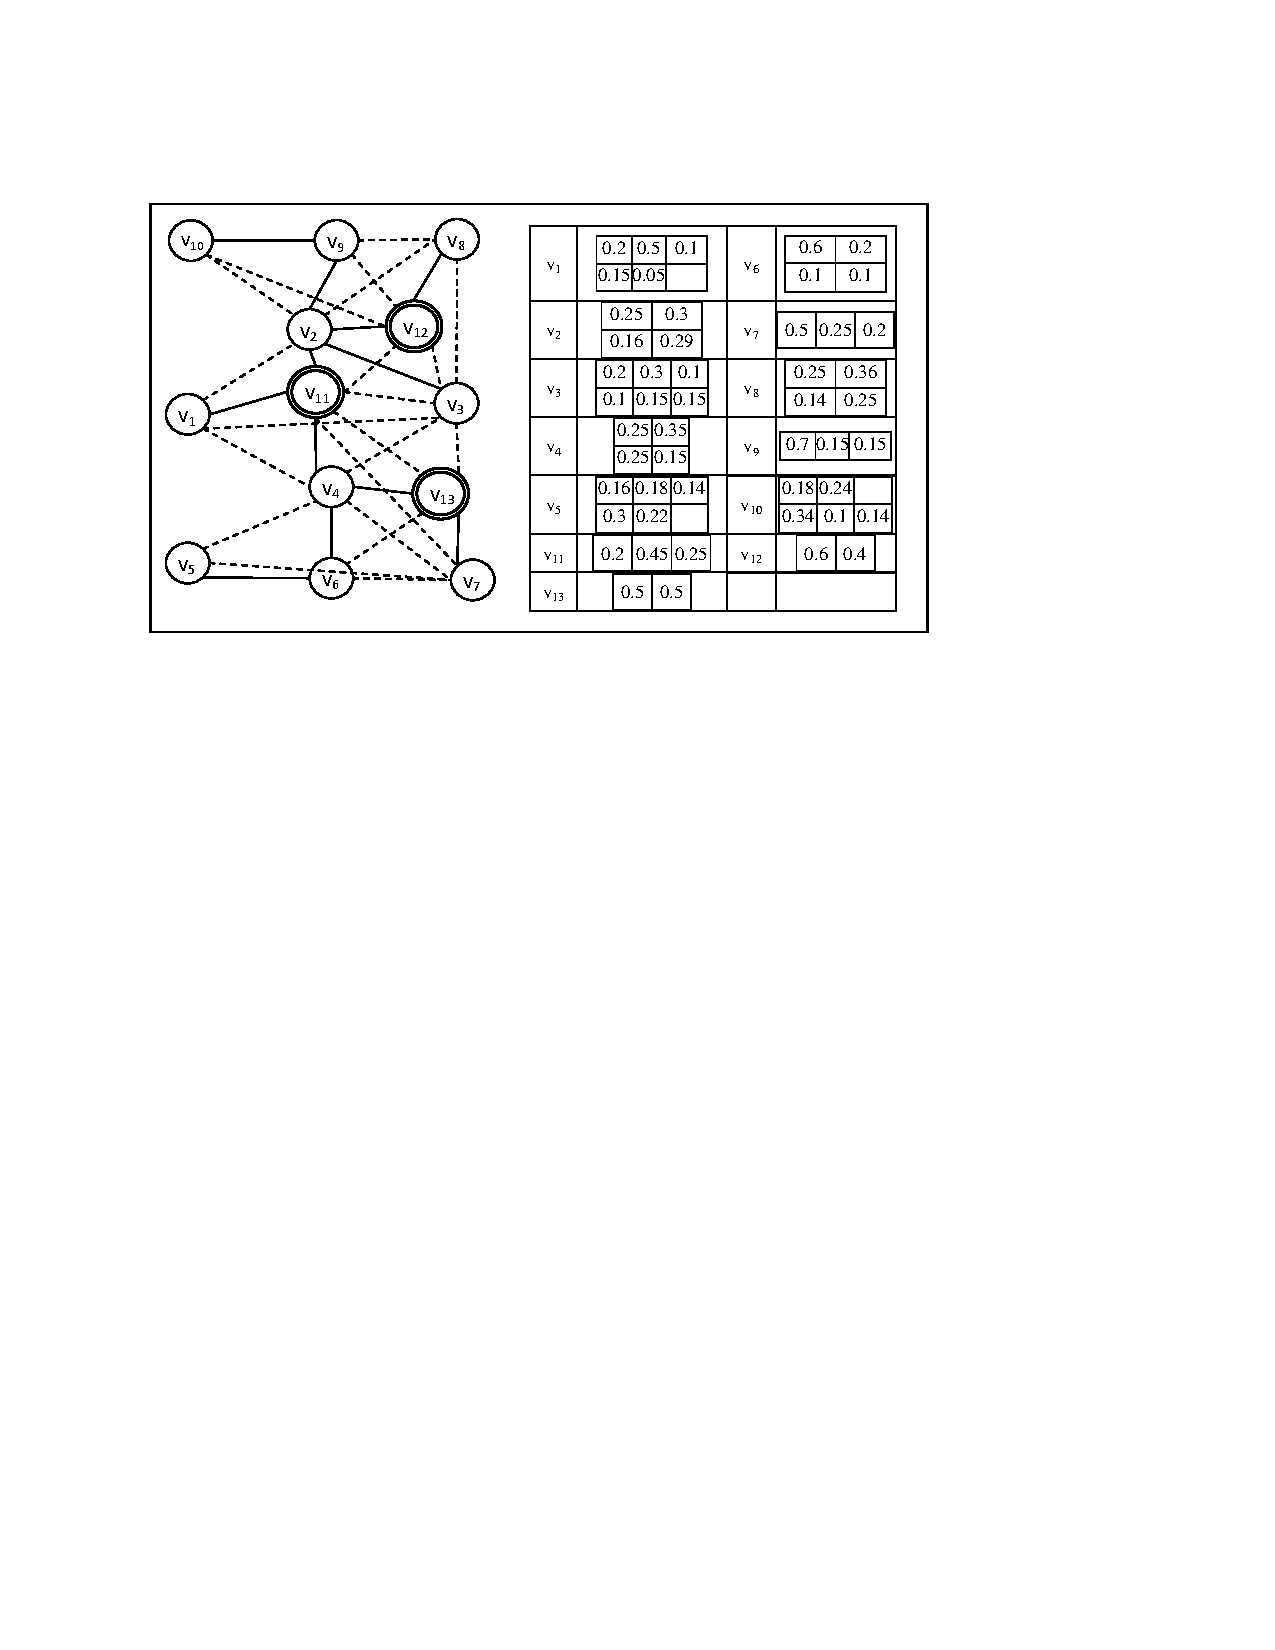
\includegraphics[width=3.3in]{g10-3r.pdf}
     %
     % \caption{A probabilistic network on 10 nodes and 3 relays}
     \caption{The $G_{10,3}$ network}
     \label{sim:g10r}
%\vspace*{-0.2in}
     \end{center}
     \end{figure}
     % ------------------------------
% ------------------------------

\nwline
{\bf 1. Running Time.}
The tree algorithm is empirically fast. The running time is typically
less than 50 millisec for the tested tree networks of size $\leq 20$ nodes.
In contrast, the exhaustive algorithm may require an hour to solve
a network of 10 nodes.

% ------------------------------

\noindent
     % ------------------------------
     %\begin{figure}[!ht]
     \begin{figure}[htbp]
     \begin{center}
     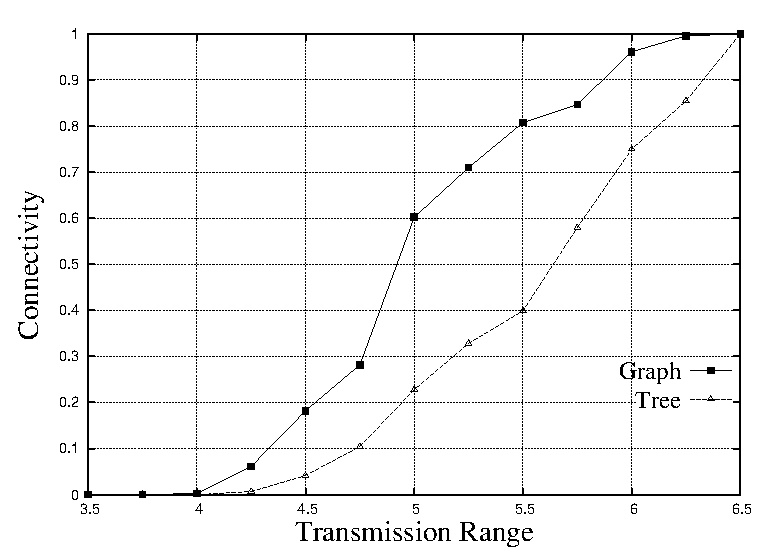
\includegraphics[width=3.0in]{conn-vs-trans.eps}
     % \caption{Exp-vs-size-pCom}
     \caption{Connectivity versus transmission range}
     \label{sim:conn:vs:trans}
%\vspace*{-0.2in}
     \end{center}
     \end{figure}
     % ------------------------------

{\bf 2. Tree bound versus exact solution for the $\ACONN$ problem.}
%
Fig.~\ref{sim:conn:vs:trans} illustrates the obtained results on $G_{10}$
when $R_{tr}$ varies in the range $[3.5,6.5]$ units.
%
Varying $R_{tr}$ in this range results in topologies with possibly
fewer links than shown in $G_{10}$.
%
When $R_{tr} \in [4.5,6.5]$, the ratio $Conn(G)/Conn(T)$ is found to be
in the range $[4.4,1]$. The ratio decreases monotonically as $R_{tr}$
increases.
%
The above finding suggests that the lower bound is more effective for
networks with good overall connectivity probability.
% ------------------------------

\noindent
     % ------------------------------
     %\begin{figure}[!ht]
     \begin{figure}[htbp]
     \begin{center}
     \includegraphics[width=3.0in]{conn-vs-nReq.eps}
     % \caption{Exp-vs-size-pSense}
     \caption{Connectivity versus $\nReq$}
     \label{sim:conn:vs:nreq}
%\vspace*{-0.2in}
     \end{center}
     \end{figure}
     % ------------------------------

{\bf 3. Tree bound versus exact solution for the $\SCONN$ problem.}
%
Fig.~\ref{sim:conn:vs:nreq} illustrates the obtained results on $G_{10}$
when $\nReq$ varies in the range $[1,10]$ nodes, and $R_{tr}= 6.5$.
%
The decreasing shape of the curves occur since increasing $\nReq$ results
in larger network states that arise with smaller probability.
%
When $\nReq$ varies in the range $[2,5]$, the ratio
$Conn(G,\nReq)/Conn(T,\nReq)$ is found to be in the range $[1.5,4.5]$.
%
The ratio deteriorates (to larger values) as $Conn(G,\nReq)$ takes small
values.
%
So, our finding here too is that the tree bound tends to be more useful
when the expected connectivity probability is relatively high.

% ------------------------------

\noindent
     % ------------------------------
     %\begin{figure}[!ht]
     \begin{figure}[htbp]
     \begin{center}
     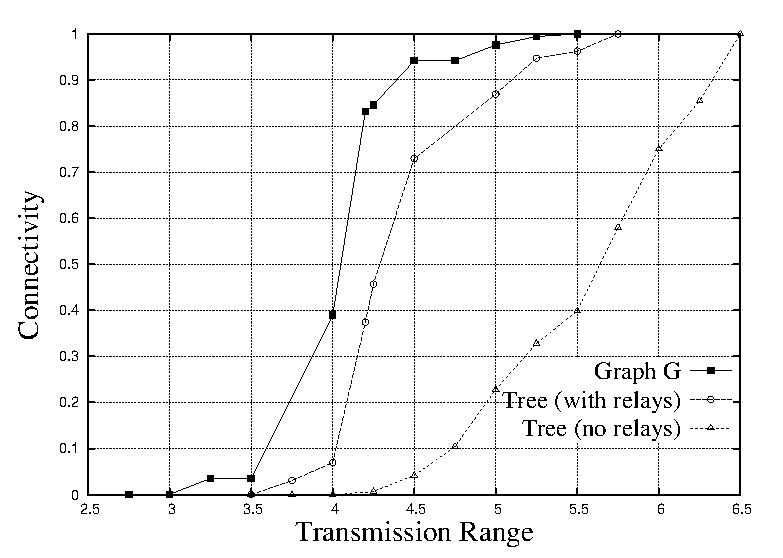
\includegraphics[width=3.0in]{conn-vs-trans-relay.eps}
     \caption{Effect of using relay nodes}
     \label{sim:conn:vs:trans:relay}
%\vspace*{-0.2in}
     \end{center}
     \end{figure}
     % ------------------------------

{\bf 4. Effect of adding relays.}
%
Deploying relay nodes can potentially increase the number of paths
from the sink node to many sensor nodes in the network.
%
Thus, the use of relay nodes can potentially improve the $Conn$ measures.
%
As it turns out, this positive effect is also reflected when using
a tree subnetwork.
%
This follows since relay nodes located in close proximity of a number
of sensor nodes can provide higher connectivity probability 
among the nodes than when removing them.
%
Fig.~\ref{sim:conn:vs:trans:relay} illustrates such positive effect
for the $\ACONN$ problem when $R_{tr}$ varies in the range $[2.5,6.5]$.
%
We have also encountered some unexpected cases where the tree bound
$Conn(T)$ of a spanning tree of a network with relays is higher
than $Conn(G)$ where $G$ is the corresponding network without relays.
%
Such findings support the positive role of using relays in UWSNs.


% ============================================================

% ------------------------------------------------------------
     % ------------------------------
%     \begin{figure*}[!ht]
%     \begin{center}
%         \subfloat[Exp-vs-size-pCom]
%         {
%          \includegraphics[width=2.2in]{exp-vs-width-pCom.eps}
%          \label{sim:exp:vs:size:pCom}
%         }
%         \iin{0.02}
         % ------------------------------
%         \subfloat[Exp-vs-size-pSense]
%         {
%          \includegraphics[width=2.2in]{exp-vs-width-pSense.eps}
%          \label{sim:exp:vs:size:pSense}
%         }
%         \iin{0.02}
         % ------------------------------
%         \subfloat[Exp-vs-Size-pCom-enhanced-cuts]
%         {
%          \includegraphics[width=2.2in]{exp-vs-size-pCom-enhanced-cuts.eps}
%          \label{sim:exp:vs:size:pCom:enhanced:cuts}
%         }
         % ------------------------------
%     \nwline
%         \subfloat[Exp-vs-Size-pSense-enhanced-cuts]
%         {
%          \includegraphics[width=2.2in]{exp-vs-size-pSense-enhanced-cuts.eps}
%          \label{sim:exp:vs:size:pSense:enhanced:cuts}
%         }
         % ------------------------------
%         \subfloat[Exp-vs-sink-location-LB]
%         {
%          \includegraphics[width=2.2in]{exp-vs-sink-location-LB.eps}
%          \label{sim:exp:vs:sink:location:LB}
%         }
         % ------------------------------
%         \subfloat[Exp-vs-Rjam-LB]
%         {
%          \includegraphics[width=2.2in]{exp-vs-Rjam-LB.eps}
%          \label{sim:exp:vs:Rjam:LB}
%         }
         % ------------------------------
%    \caption{Simulation Results}
%    \end{center}
%    \vspace{-0.3in}
%    \end{figure*}
    % ------------------------------

% ------------------------------------------------------------




% ------------------------------------------------------------
\section {Concluding Remarks}
%
Quantifying the likelihood that a sufficient number of sensor nodes
is connected to a sink node in a given UWSN is a challenging problem for
networks with semi-mobile and mobile nodes.
%
Our work here adopts a flexible probabilistic graph model to formulate
a class of parameterized network connectivity problems.
%
The problem setting allows the network to utilize both sensor nodes
and relay nodes.
%
For scenarios where the model is exact, we show that the exact
probabilistic connectivity can be computed efficiently for tree-like
networks.
%
Our simulation results show the usefulness of the algorithm in
computing efficient lower bounds on the solution of any arbitrary
network. Scenarios with deployed relay nodes are also analyzed.
%
Future work will consider obtaining stronger bounds of the formulated
problems.

% ------------------------------------------------------------

%\nwline
%\centerline{\sc Acknowledgment}
%\section*{Acknowledgment}
% This research is supported by NSERC Canada.
% ------------------------------------------------------------
%	\newpage

% Styles: latex8, unsrt, IEEEtranS.bst
%
\bibliographystyle{IEEEtran}
\bibliography{tree-UWSN}

%% \bibliography{exposure,00bib/mypapers,00bib/wireless-sensor,00bib/rel}

%% \bibliography{00bib/mypapers,00bib/qos,00bib/rel,00bib/general,00bib/wireless-sensor}

% ============================================================
\end{document}
